
%(BEGIN_QUESTION)
% Copyright 2010, Tony R. Kuphaldt, released under the Creative Commons Attribution License (v 1.0)
% This means you may do almost anything with this work of mine, so long as you give me proper credit

Sketch the wires necessary to complete this start/stop motor control circuit, including proper connection of the overload (OL) contact.  Note that the contactor coil operates on 120 volts (not 480), so you will need to wire in the control power transformer.  Also, you will need to make the motor control circuit {\it latch} so that it continues to run after the ``Start'' switch is released:

$$\includegraphics[width=15.5cm]{i03686x01.eps}$$

Then, explain how to make the motor spin in the opposite direction, if it is discovered upon initial testing that the motor spins the wrong way for the machine it is supposed to power.

\underbar{file i03686}
%(END_QUESTION)





%(BEGIN_ANSWER)

This is one possible answer:

$$\includegraphics[width=15.5cm]{i03686x02.eps}$$

\vskip 10pt

To reverse rotation, swap any two of the three-phase lines.  This may be done at the source (L1-L3), at the motor (T1-T3), or anywhere in between.

\vskip 10pt

I recommend half credit for proper wiring, and half credit for properly identifying how to reverse rotation.

%(END_ANSWER)





%(BEGIN_NOTES)

{\bf This question is intended for exams only and not worksheets!}.

%(END_NOTES)

